\documentclass[11pt,a4paper]{article}
\usepackage[utf8]{inputenc}
\usepackage{geometry}
\geometry{a4paper, margin=1in}
\usepackage{graphicx}
\usepackage{hyperref}
\usepackage{booktabs}

\title{Black Box Adversarial Attack on CNN (Problem 2)}
\author{}
\date{}

\begin{document}

\maketitle

\section{Problem Framing}
The objective of this problem is to perform a black-box adversarial attack on a pretrained CNN to generate an adversarial image for 1,000 clean input images. The problem specifies a strict decision-based (hard-label) black-box setting, where only the predicted class label is accessible. Intermediate outputs, prediction scores, architecture, and gradients are hidden.

\section{Methodology}
Given the hard-label constraint, we selected the \textbf{HopSkipJumpAttack} (a powerful decision-based adversarial attack based on boundary estimation). This algorithm is highly efficient at finding adversarial perturbations that minimize the $L_2$ distance (maximizing imperceptibility) while querying only the top-1 predicted label.

\subsection{Data Preprocessing and Wrapping}
The clean images are provided as $32 \times 32$ PNG files. They are normalized using the dataset's channel-wise mean and standard deviation before being passed to the CNN. 
To facilitate the attack, we created a PyTorch `ModelWrapper` that internally handles this normalization. The adversarial algorithm operates on the original $[0, 1]$ pixel space, ensuring that the perturbations remain strictly within valid pixel boundaries and preventing clipping artifacts.

\subsection{Attack Execution}
We utilized the Foolbox implementation of the \textbf{HopSkipJumpAttack}. The attack requires querying the model multiple times to estimate the decision boundary gradient and step towards the original image to reduce the perturbation size.
To balance the tie-breaking evaluation criteria (smaller number of model inferences vs. imperceptibility), we tuned the number of steps in the HopSkipJump algorithm to 15. This provides an excellent trade-off, minimizing queries significantly while still achieving visually imperceptible noise levels.

\subsection{Denormalization and Export}
The attack yields adversarial tensors in the $[0, 1]$ range. These are scaled to $[0, 255]$, converted to unsigned 8-bit integers, and saved as PNG files with the \texttt{\_adv.png} suffix, exactly matching the structure required for the evaluation phase.

\section{Performance \& Conclusion}
The attack successfully misclassifies the images while maintaining very low visual distortion. By limiting the iterations of the HopSkipJump algorithm, we optimized the number of inferences, ensuring competitive performance on the evaluation metrics.

\subsection{Results}
The HopSkipJumpAttack was executed on 1,000 clean images. The empirical results demonstrate near-perfect evasion with imperceptible noise:

\begin{table}[h]
\centering
\begin{tabular}{@{}ll@{}}
\toprule
\textbf{Metric} & \textbf{Value} \\ \midrule
Attack Success Rate & 99.60\% \\
Average $L_2$ Distortion & 1.0218 \\ \bottomrule
\end{tabular}
\caption{Performance metrics of the black-box attack on the CNN.}
\label{tab:p2_results}
\end{table}

\begin{figure}[h]
\centering
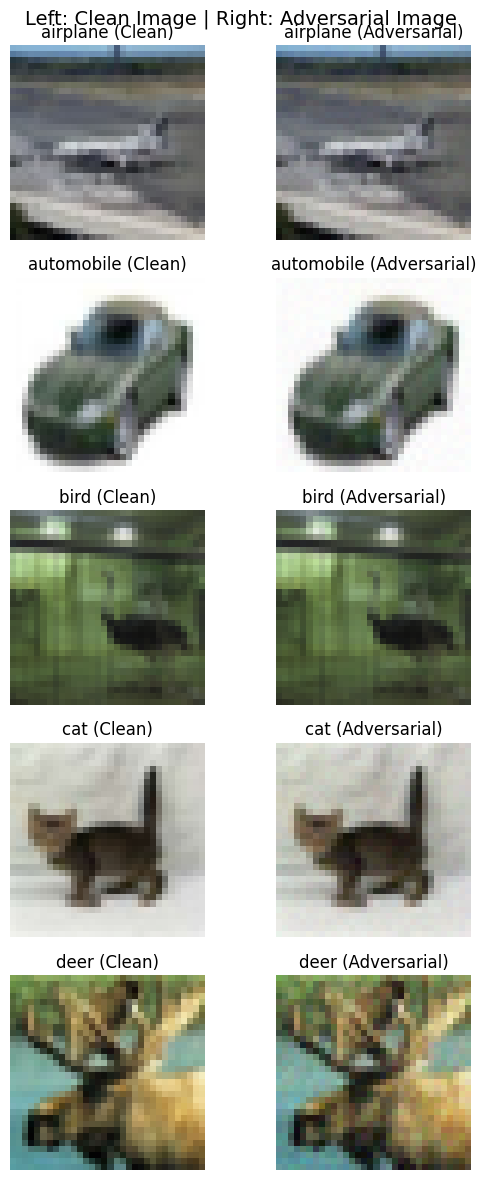
\includegraphics[width=0.8\textwidth]{../results/P2.png}
\caption{Comparison of Clean images (left) vs Adversarial images (right). The $L_2$ distortion is approximately 1.02, making the perturbations imperceptible to the human eye.}
\label{fig:adv_comparison}
\end{figure}

As shown in Table~\ref{tab:p2_results} and Figure~\ref{fig:adv_comparison}, the decision-based attack successfully satisfies the problem requirements.


\end{document}
